\chapter{调试通道总体设计与关键技术}

\section{总体设计}
	在嵌入式软件的开发、移植、运行时都需要输出一些调试或日志信息,目前VxWorks当中使用WorkBench集成开发平台来完成软件的开发、调试工作,它所使用的调试方式是一种典型的在线调试方式,但是在项目的实际生产环境当中他们希望使用一种离线的调试日志的方式来进行程序的调试工作,它们希望在设备运行的大量应用程序当中加入调试信息,这些程序的调试信息都能够自动的传输到普通的PC上,他们能够在之后查看其调试信息,对这些信息分析工作。
	
	基于以上的需求,此次我们的工作就是在VxWorks下完成一个能够满足他们的需求的调试通道,在主机端我们使用一个分析程序来对目标机上传输过来的调试数据进行分析;在目标机端我们给应用程序提供一个调试接口,将调试信息从通信接口中传输出去,本次设计的调试通道主要应用于VxWorks下程序移植时大量调试信息的输出的场景。对于在该应用场景下的整个调试通道的框架如\autoref{fig:sys-data-diagram}所示。

\begin{figure}[!h]
\centering
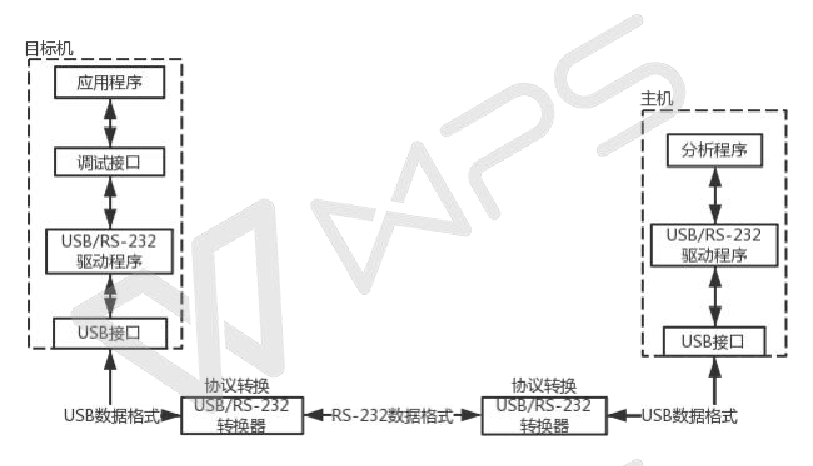
\includegraphics[width=1.0\textwidth]{./graphics/sys-data-diagram.pdf}
\caption{调试通道框架图}\label{fig:sys-data-diagram}
\end{figure}

	在我们所设计的调试通道当中,目标机上的上层应用程序会调用调试通道中所提供的调试接口,通过调试接口将调试信息传递给通信接口,由于设备上没有可用的RS-232串口,而USB的体系结构又是主从式的,无法直接作为调试通道的通信接口来使用,为了解决这个问题,在我们的调试通道当中使用外部的USB/RS-232的转换器来实现通信接口,同时在系统上使用与设备相对应的USB/RS-232设备驱动程序。这样PC端的应用软件应用软件仍然是针对RS-232串行端口编程的,外设也是以RS-232为数据通信通道的,但是PC端到外设之间的物理连接却是USB总线,其上的数据格式也是USB数据格式。
	
	在VXWorks中并没有现成可用的USB转串口驱动以及USB转串口转换器,所以我们需要自己选择一个外部的USB/RS-232转换器,以及针对该USB/RS-232转换器的USB转串口驱动。在主机端都会有已经实现好的USB转串口驱动程序,我们只需要提供转换器即可,这样用户在不需要理会USB的复杂的内部协议的情况下来享受USB接口的即插即用、数据可靠传输、扩展方便等优点。分析程序会自动接收串口的数据,完成协议分析、调试信息的定位等工作。
\begin{figure}[!h]
\centering
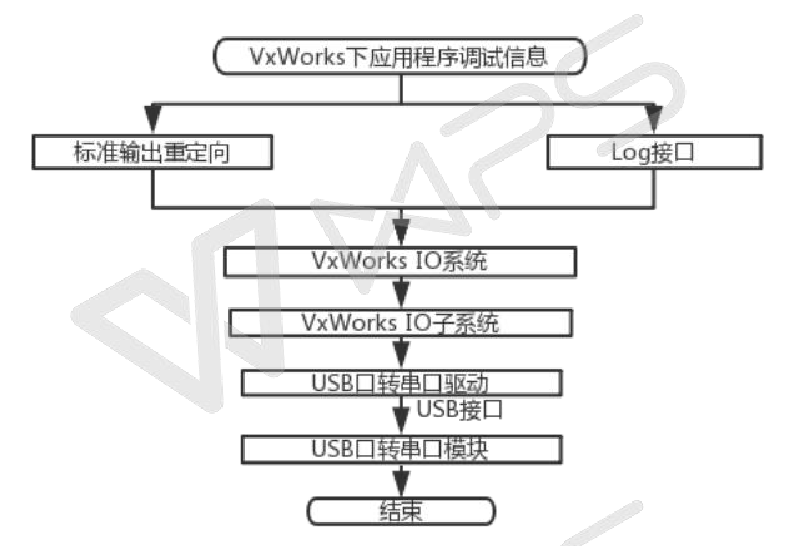
\includegraphics[width=1.0\textwidth]{./graphics/debug-system-diagram.pdf}
\caption{目标机调试通道层次结构图}\label{fig:debug-system-diagram}
\end{figure}
	
	对于目标机上的调试通道的结构如\autoref{fig:debug-system-diagram}所示。在VxWorks当中I/O 系统和I/O子系统是作为操作系统的重要组成部分已经实现好了的,我们的调试通道所需要设计的部分主要是接口模块和USB口转串口模块。
	
	提供给应用层的接口模块负责将系统应用层的输出通过我们的USB口转串口驱动程序传输到windows PC机,输出的形式包括特定内容的格式化的输出和普通的重定向的输出,格式化的输出我们会使用自定义的Log接口进行格式控制,为此我们设计了一个自定义的Log协议格式,其中的内容包含有调试级别、调试信息所在的文件、调试信息所处的行号、输出该条调试信息的时间等;重定向的输出包括RTP模式下的重定向和task模式下的重定向,VxWorks中对于这两种模式需要使用不同的重定向方式。
	
	USB口转串口模块用于在VxWorks上实现一个USB口转串口驱动程序,负责将上层应用的信息传输到windows PC,包括一个特定需求的驱动程序的实现和一个普通的驱动程序的实现。对于本次特殊需求的驱动程序相对于普通的驱动程序而言在流程和结构上进行了修改,以使其达到特定的要求,具体的实现我们会在第三节进行介绍。两种实现方式中都会包含有驱动程序加载、卸载模块,设备的打开、关闭、读、写、控制模块。同时在驱动程序中还需要一个数据的管理模块,我们会使用循环缓冲区来管理数据。


	


\section{关键技术}

\subsection{VxWorks驱动开发}
	
	在VxWorks当中使用I/O子系统来管理设备驱动,I/O 子系统在整个VxWorks当中起着承上启下的作用,各种类型的设备都必须要向I/O子系统进行注册才能够被内核访问,I/O子系统在VxWorks当中的作用是维护系统设备表、系统驱动表、系统文件描述符表\cite{VxWorks内核解读}\cite{曹桂平2011VxWorks}。设备驱动在VxWorks中就靠这三个数据结构来进行管理,所以对于设备驱动而言非常重要。设备驱动程序初始化时会对硬件完成初始化的配置,同时会向I/O子系统注册自己,注册之后I/O子系统才能找到该驱动。

\noindent \textbf{1. 系统设备表}

	系统设备表是VxWorks中为了管理系统上的所有设备而使用的一个链表,系统设备表中每一个节点都是一个DEV\_ HDR类型的结构体,系统会将每个设备DEV\_ HDR连接在如\autoref{fig:VxWorks系统设备示意图}所示的系统设备表中。DEV\_ HDR是wind内核规定的每一个设备都必须要具有的一个数据结构,且必须是设备自定义结构的第一个成员,之后系统只会使用这个结构来代表该设备。DEV\_ HDR结构体当中只包含有三个成员:一个设备链表节点;一个设备驱动号;一个指向设备名的指针。
	其定义如\autoref{fig:DEVHDR} 所示。

\begin{figure}[!h]
\centering
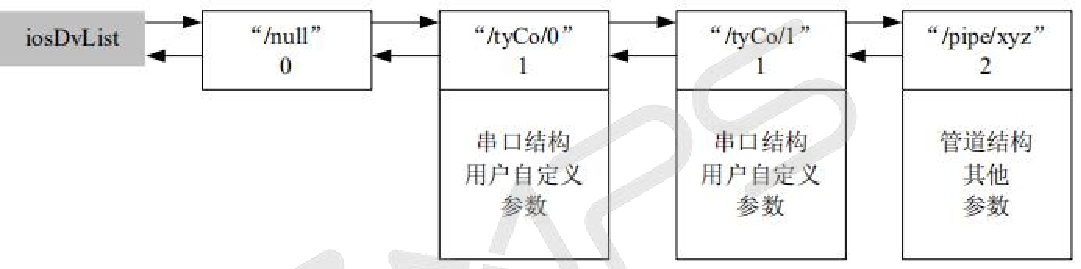
\includegraphics[width=1.0\textwidth]{./graphics/vxworks-device-link.pdf}
\caption{VxWorks系统设备示意图}\label{fig:VxWorks系统设备示意图}
\end{figure}
	
\begin{figure}[!h]
\centering
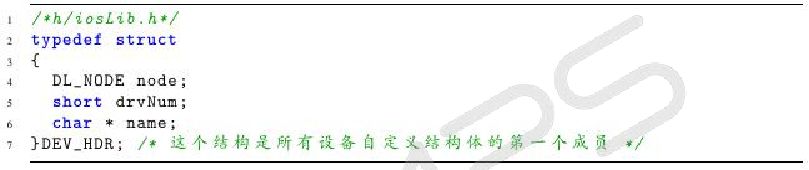
\includegraphics[width=1.0\textwidth]{./graphics/DEVHDR.pdf}
\caption{DEV\_ HDR结构体}\label{fig:DEVHDR}
\end{figure}

同时VxWorks系统提供了一个设备的注册函数iosDevAdd( DEV\_ HDR *pDevHdr, char *name, int drvnum),该函数用来将一个设备添加到系统设备表当中,系统设备表在每次添加设备时就会在表中增加一个节点表示该设备,删除设备时就会将该设备的节点从表中删除,一个设备添加到系统之后,就可以使用open()函数对其进行操作,open()会通过将传递过来的设备名与系统设备表当中进行设备名匹配来完成设备的打开操作,匹配的原则是最佳匹配,匹配成功之后就可以实现文件与设备的连接\cite{刘小军2008基于},之后就可以使用相对应的注册的设备驱动进行其他的文件操作。

\noindent \textbf{2. 系统驱动表}


	系统驱动表用于管理当前注册到I/O子系统下的所有驱动程序,既可以是直接驱动硬件工作的驱动程序,也可以是注册到I/O子系统下的驱动中间层\cite{VxWorks内核解读}。
	在VxWorks中系统驱动表的底层实现是一个数组,数组中的每一个元素就是一个系统驱动表的表项,每一个表项都是一个 DRV\_ ENTRY 类型的结构体,该结构定义在内核的头文件iosLibP.h当中,其定义如\autoref{fig:DEVENTRY}所示。
	
\begin{figure}[!h]
\centering
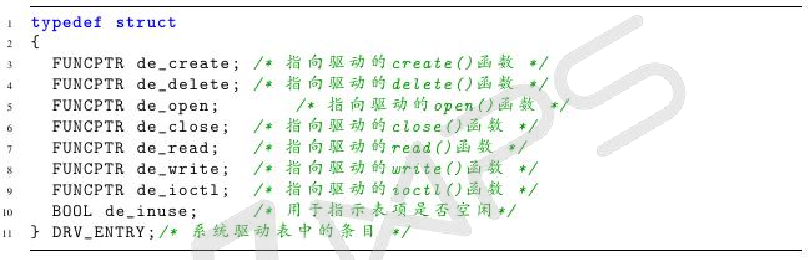
\includegraphics[width=1.0\textwidth]{./graphics/DEVENTRY.pdf}
\caption{DEV\_ ENTRY结构体}\label{fig:DEVENTRY}
\end{figure}

	DEV\_ ENTRY结构体当中的大多数成员都是函数指针,他们用于指向所注册的驱动程序中的一个用于完成特定功能的实际函数,这些函数的功能要符合IO系统预定义好的规则,这些函数被加入到系统驱动表中之后就可以完成与用户层提供的标准函数接口对接\cite{VxWorks内核解读}\cite{VxWorksDriverAPI}\cite{Wind2003VxWorks}。在DEV\_ ENTRY结构体当中唯一不是函数指针的成员是一个布尔类型的 de\_ inuse 成员,若该成员为FALSE则表示该表项目前是未被使用的状态,即该表项没有被任何的驱动所注册。

	VxWorks当中给我们提供了一个驱动的注册函数iosDrvInstall(),使用该函数注册我们的驱动之后,系统驱动表就会分配一个未被使用的表项给该驱动,然后使用iosDrvInstall()所提供的的参数来填充系统驱动表当中的指针,并将de\_ inuse置为TRUE的状态,一个驱动程序不需要实现所有的IO函数,对于实现的函数,在注册时直接将其指针置为NULL即可。

\noindent \textbf{3. 系统描述符表}

	系统描述符表用于管理当前系统中所打开的所有文件描述符,VxWorks中系统描述符表的底层实现也是一个数组。每次执行open()调用成功之后,系统就需要从系统描述符表中分配一个表项给程序使用,并将文件描述符的表项索引作为文件描述符的ID返回给应用程序。之后应用程序直接通过这个ID就可以对文件进行操控,无需每次都是用文件名。
	在VxWorks中,标准输入、标准输出、标准错误输出虽然使用 0,1,2 三个文件描述符来表示,但是它在底层的实现上可能并不是占用了三个文件描述符表的表项,而是只占用一个表项,即三个文件描述符指向同一个文件描述符的表项\cite{VxWorks内核解读}\cite{An2003Implementation},这一点是需要注意的。
		
	
系统文件描述符表中每一个表项都使用 FD\_ ENTRY 这个结构体来表示,这个结构定义在内核的头文件iosLibP.h 中,其定义如\autoref{fig:FDENTRY}所示。


\begin{figure}[!h]
\centering
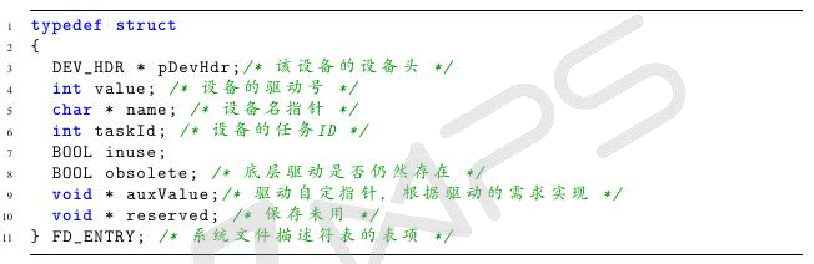
\includegraphics[width=1.0\textwidth]{./graphics/FDENTRY.pdf}
\caption{FD\_ ENTRY结构体}\label{fig:FDENTRY}
\end{figure}

用户的应用程序每次使用open()系统调用系统文件描述符表中就会增加一个有效表项,该表项的FD\_ ENTRY结构体会根据open()调用的内容来进行填充,每一个文件能够进行的open()调用是有限制的,因为数组的容量是固定的,每个驱动的FD\_ ENTRY结构数组满了之后就无法再对这个设备进行open()操作,此时 open()函数将会失败返回\cite{VxWorks内核解读}。系统会在表中的索引偏移 3 (0、1、2被系统占用)之后找一个最先找到的未使用的id作为文件描述符返回给用户。




	
\subsection{VxWorks 中的信号量机制}
	
	任务间的通信机制用于协调多个任务之间的活动,VxWorks内核当中为我们提供了丰富的任务间通信机制,包括共享内存、信号量、消息队列、管道、信号、Sockets等\cite{胡明民2012基于实时操作系统}\cite{冯云贺2014基于}。在我们调试通道的信息传输中需要设计一个特殊需求的USB转串口驱动,在驱动当中需要使用信号量机制
	来确保对驱动内部缓冲区中的数据正确、有序的读写,因此我们有必要先了解一下VxWorks下的信号量机制。

	
	信号量是一种在程序的设计当中最常使用的通信机制,其主要作用是线程间的同步和互斥。VxWorks中提供POSIX信号量的同时还设计了专门的wind信号量,POSIX信号量的使用主要是为了方便程序的移植。
	和POSIX信号量的不同之处在于,VxWorks中设计的wind信号量为VxWorks系统进行了高度的优化,使得其更适用于实时操作系统,能够更快的实现任务间通信。VxWorks中信号量是一个指向SEMAPHORE类型的结构指针,提供了二进制信号量、互斥信号量、计数信号量三种类型的信号量机制,他们适用于解决不同类型的问题。
	
\begin{itemize}
\item 二进制信号量\\
	二进制信号量是最快、最通用的信号量,既可以用于同步也可以用于资源计数。wind的二进制信号量所需系统开销最少,适用于高性能的需求。二进制信号量在资源可用时标记为FULL,在资源不可用时标记为EMPTY。在VxWorks中二进制信号量使用函数semBCreate()来创建,二进制信号量的提取和释放过程如\autoref{fig:erjinzhiTiQu}和\autoref{fig:erjinzhiShiFang}所示。

\begin{figure}[!h]
\centering
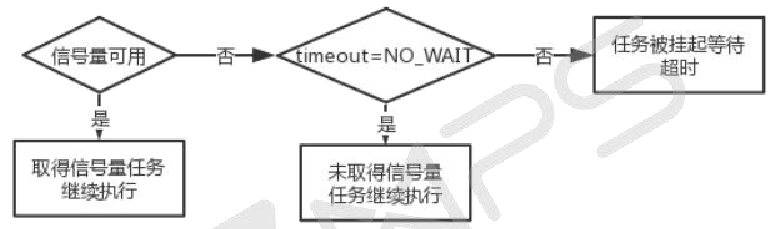
\includegraphics[width=13cm , height=10cm]{./graphics/erjinzhiTiQu.pdf}
  \caption{提取信号量}\label{fig:erjinzhiTiQu}
\end{figure}

\begin{figure}[!h]
\centering
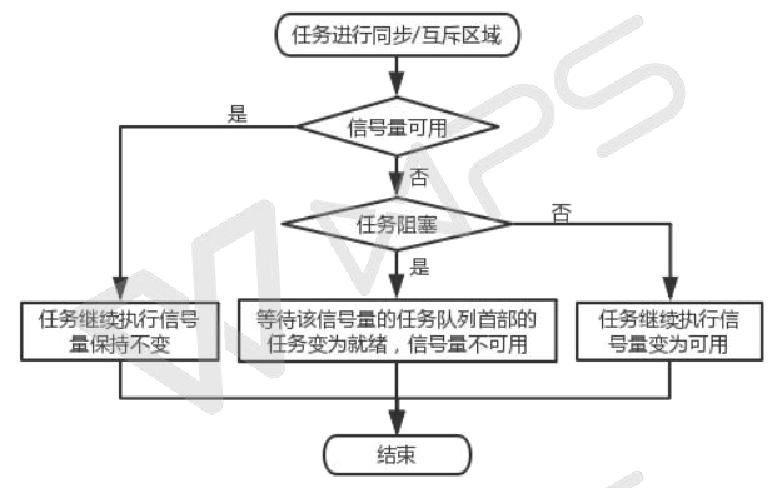
\includegraphics[width=13cm , height=10cm]{./graphics/erjinzhiShiFang.pdf}
  \caption{释放信号量}\label{fig:erjinzhiShiFang}
\end{figure}


\item 互斥信号量\\
	互斥信号量可以看做是一种特殊的二进制信号量(资源数为1),它优化了互斥、优先级继承、删除安全等问题,这使得它能够更好的服务于任务间的互斥需求;互斥信号量的基本行为和二进制信号量是一致的,但是互斥信号量只能够用于互斥,不能够用于同步,该信号量只能够由获得的该信号量的进程来进行释放,不能够由其它的进程进行释放。它使用SEM\_ INVERSION\_ SAFE和SEM\_ Q\_ PRIORITY选项来使得该信号量能继承优先级算法,以此解决优先级的倒置问题;使用SEM\_ DELETE\_ SAFE选项来解决删除安全问题,在VxWorks中互斥信号量使用系统提供的semMCreate()函数来创建;
	
\item 资源计数信号量\\
	资源计数信号量也是一种特殊的二进制信号量(资源数较多),它会跟踪信号量增加、删除的次数,每次释放一个信号量,内部的计数器就会执行加一操作,每次提取一个信号量,内部的计数器就会执行减一操作,当计数器为0时,表示没有可供使用的资源,此时提取信号量的操作就会被阻塞,在VxWorks中资源计数信号量使用系统提供的semCCreate()函数来创建。

\end{itemize}
	
三种信号量的释放操作都是使用semGive()函数;提取操作都是使用semTake()函数,在提取信号量是我们可以选择是否允许超时,超时可以作为解决阻塞的一种方法。



\subsection{USB技术}
	USB(Universial Serial Bus)作为PC领域的最新型的接口技术,目前已被各个PC厂家所支持,并且在各类外设当中都广泛的采用USB接口。USB的开发技术也已经很成熟,通用串行总线开发者论坛(USB Implementers Forum,USB IF)目前制定了三种USB接口标准:USB1.1,USB2.0和USB3.0。USB采用菊花链的形式连接所有的设备,最多可以连接127个设备,USB的总线拓扑结构如\autoref{fig:USB体系结构}所示
\begin{figure}[!h]
\centering
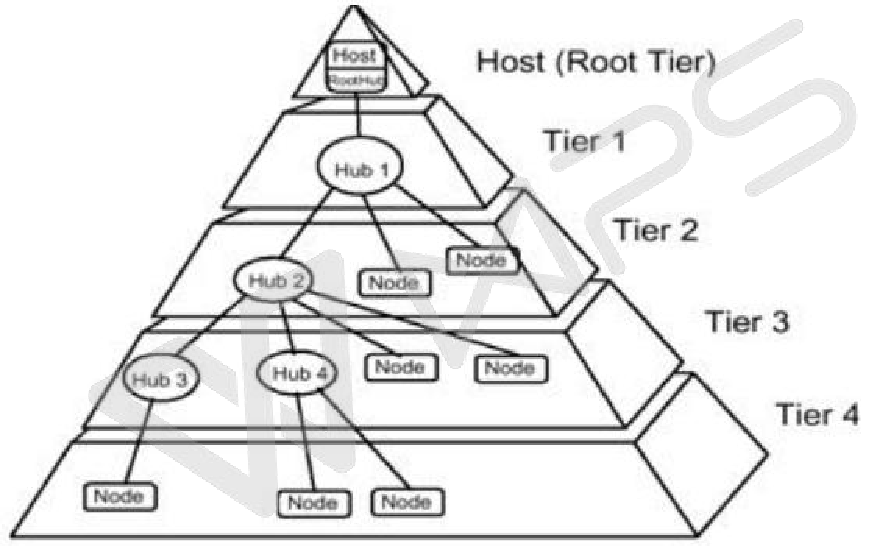
\includegraphics[width=1.0\textwidth]{./graphics/usb-structure.pdf}
\caption{USB总线拓扑结构}\label{fig:USB体系结构}
\end{figure}


USB的体系结构由三个部分组成,分别是USB主机(Host)、USB集线器(Hub)、USB设备(Device)。其中我们需要了解的关键部分是USB主机和USB设备。

\\
	
\noindent \textbf{1. USB主机}
	
	USB主机是USB体系中的核心,且系统中只允许一个USB主机存在。USB主机上的USB接口是USB主控制器,其控制着总线上所有USB设备数据通信。对于USB的体系结构而言,其数据的传输都是USB主机端发起的,非主机端(设备端)只能够被动的进行响应。USB主机需要完成的功能包括检测设备的热插拔、管理主机和设备之间的信息(控制和数据)流\cite{李雪红2004USB}\cite{莫宏伟2001USB}。


\\

\noindent \textbf{2. USB设备}

	USB设备指的是提供具体功能的而外部USB设备,是相对USB主机而言的,它们受USB主机的控制,只能对主机的请求进行被动响应。USB主机端会在检测到USB设备的动作之后会通过默认管道和USB设备进行通信,对其进行必要的初始化配置,并给设备提供适合的驱动程序(如果有的话),一个USB设备会通常会有很多的属性,它会通过这些属性来完成主机的配置要求。一些USB设备的属性如下:
	\begin{itemize}
	\item \textbf{描述符(Descriptor)属性}\\
	描述符是USB协议中定义的一套用来描述USB设备的功能和属性的固定结构,我们可以通过描述符了解设备的各种属性,描述符又分为设备描述符、配置描述符、接口描述符、端点描述符、字符串描述符\cite{张杰2008基于}\cite{边海龙2004USB}除此之外,设备还可以提供自己专用的描述符,分为设备类描述符和供应商自定义描述符,我们使用的USB口转串口设备就不属于一个标准的USB设备,它会为我们提供供应商自定义的描述符,我们使用需要使用它来对设备进行识别。
	
	\item \textbf{类(Class)属性}\\
	由于USB协议支持许多的外围设备,而这些设备又可以根据功能来分成一些相近的类,如打印机类、键盘类等。这样主机端就可以为这些功能相近的设备提供一个类驱动,类驱动可以用于驱动所有属于同一类的设备,不需要再为每一个设备提供一个完整的驱动程序。这大大的方便的设备的制造商,他们的设备只需要符合某一类的驱动,就可以使用该类驱动程序来驱动其设备,之后只需要实现简单的包含有设备特性的客户端驱动即可,若设备没有特殊的特性,则直接使用类驱动即可\cite{李雪红2004USB}。	
	
	\item \textbf{功能(Function)/接口(Interface)属性}\\
	功能或接口是USB协议中定义的设备的某种能力,Function是从功能角度来说的,从设备的角度来说,被称为Interface。对于一个设备他可以拥有很多个不同的接口,每一个接口负责完成设备的一个特定的功能,并且这个接口具体实现什么样的功能并不是固定的,当USB设备处于可配置状态的时候能够通过控制命令来改变某一个接口的功能,一个接口能够具有什么样的功能会在USB的接口描述符中进行描述。
	
	\item \textbf{端点(Endpoint)属性}\\
	端点是USB设备与USB主机逻辑上的通信流的终点,每个设备都拥有一个可独立进行操作的端点集合,且每个端点在使用时都要先初始化其数据传输方向(IN/OUT),即使端点号相同但是传输方向不同的通信点也是不同的端点\cite{李雪红2004USB}。
	
	\item \textbf{管道}\\
	管道可以看做是设备上的一个端点和主机上的软件的联合体,设备和主机间的数据传输要基于管道进行。在USB的通信过程中首先要建立一个管道才能够进行数据的传输,USB设备在和主机通信时都会建立一个默认的管道,这个管道对应的端点是默认端点0,之后需要自己使用其它的端点来建立我们的数据传输过程中需要使用的输入或输出管道。在我们的USB口转串口驱动中会为每一个设备建立两个管道,一个批量输出管道和一个批量输入管道。
	
	\item \textbf{设备地址}\\
	设备地址用于区分USB系统中的一个USB设备的特殊标识,设备地址会在设备初始化之后由主机进行分配且是唯一的。设备地址单元共有7bit,其中地址0是缺省地址,在设备初始化的时候使用,理论上系统可以区分127个USB设备\cite{李雪红2004USB}。
	\end{itemize}	



\noindent USB规范规定了USB主从设备之间的四种传输方式,每种方式有各自的用途\cite{USB总线接口开发指南}:

\begin{itemize}
\item \hei{控制传输}:控制传输USB传输方式中最重要、最复杂的一种,它适用于少量、对时间和速率无要求的场合,一个USB设备插入主机之后就是使用这种传输方式来读取设备的地址和描述符等信息。所有的设备都会在其0号端点的缺省管道当中支持控制传输\cite{张杰2008基于}。
\item \hei{批量传输}:批量传输有两种最基本的事物类型:BULK\_ IN和BULK\_ OUT,其主要用于处理对数据传输速率不是很高的情况,批量传输使我们的USB口转串口设备所使用的主要传输传输方式,每次有数据需要传输时我们都会构建一个IRP使用批量传输将其传出或传入。
\item \hei{中断传输}:中断传输也有两种基本的事务:IN和OUT,其主要是为那些要快速实现主机和设备的交互,但是数据量很小、对服务时间有要求的情况而准备的。
\item \hei{等时传输}:等时传输也是由基本的IN和OUT两种事务组成,主要用于处理大量、恒速、对时间周期有要求的数据。等时传输只有全速和高速设备才支持,低速设备不支持\cite{张杰2008基于}。
\end{itemize}


	

\section{本章小结}
	本章重点介绍了本次的VxWorks调试通道的整体架构,并介绍了介绍了各个部分的设计方案,最后介绍了在本次的设计当中所需要使用关键技术和所需了解的重要知识,主要包括VxWorks下的驱动开发必须的结构、驱动中所需使用的VxWorks的通信机制、缓冲区技术、USB技术。下面将要讨论VxWorks下的调试通道的详细的设计细节和具体的实际机制。

























